\newpage
\appendix
\chapter{Appendix Part I}
\section{Figures and graphs}


\section{Proofs}

\subsection{\cref{lem:composition_lemma}: Composition Lemma for $\wlnn$}\label{app:composition_proof}
Before we begin with the actual compositon proof, we give a formal defintion and notation for MLPs.

\begin{definition}[Multilayer Perceptron]\label{def:mlp}
    Multilayer perceptrons are a class of functions from $\Rb^n$ to $\Rb^m$, with $n,m \in \Nb$. In this thesis, we define a multilayer perceptron as a finite sequence, such that a multilayer perceptron $\mlp$ is defined as $\mlp \coloneqq (\mlp)_{i\in[k]}$ where $k$ is the number of layers. For every $i \in [k]$, the $i$.th layer of the $\mlp$ is the $i$.th item in the finite sequence $\mlp_i$. Further, all layers are recursively defined as: \todo{Adapt the notation for sequences $(\mlp_i)_{i \in [k]}$}
    \begin{align*}
        \mlp_{0}(v) &\coloneqq v\\
        \mlp_{i+1}(v) &\coloneqq \sigma_i(W_i \cdot \mlp_{i} (v) + b_i), \quad \forall i \in [k-1]
    \end{align*}
    where $\sigma_i$ is an element wise activation function, $W_i$ is the weight matrix and $b_i$ the bias vector of layer $i$. Note, that for each $W_i$, the succeeding $W_{i+1}$ must have the same number of columns as $W_i$ has rows, in order to be well-defined. Similarly, for every layer $i$, $W_i$ and $b_i$ have to have the same number of rows.
    Following this definition, when applying a $\mlp$ on input $v \in \Rb^n$ it is $\mlp(v) \coloneqq (\mlp)_k(v)$.
\end{definition}

\begin{proof}[Proof of \cref{lem:composition_lemma}]
    Let $\cC$ be a collection of functions computed by $\wlnn$, $h_1, \dots ,h_n \in \cC$, and $\mlp^\bullet$ a multilayer perceptron. Further, let $f_{1}, \ldots, f_{n}$ be the encoding functions, as well as $\text{MLP}_1, \ldots, \text{MLP}_n$ be the multilayer perceptrons used by $h_1, \dots h_n$ respectively. As outlined above, we will now construct $f^*$ and $\mlp^*$, such that for all graphs $G \in \cX$:
    \begin{equation*}
        \mlp^\bullet(h_1(G), \dots ,h_n(G)) = \mlp^* \circ f^* (\MSopen \wl(G)(v) \mid v \in V(G) \MSclose)
    \end{equation*}
    with which we can conclude that the composition of multiple functions computable by $\wlnn$, is in fact also $\wlnn$ computable. 

    We define the new encoding function $f^*$ to work as follows on an arbitrary input multiset $M$:
    \begin{equation*}
        f^*(M) := \textsf{concat}(
            \begin{bmatrix}
                f_1(M)\\
                \vdots\\
                f_n(M)
            \end{bmatrix}),
    \end{equation*}
    where $\textsf{conccat}$ is the concatenation function, concatenating all encoding vectors to one single vector.

   Using the decomposition introduced in \cref{def:mlp}, we can decompose each $\mlp_i$ for $i \in [n]$ at layer $j > 0$ as follows: $(\mlp_i)_{j}(v) := \sigma_{i,t}(W^{i}_{j} \cdot (\mlp_i)_{j-1}(v) + b^i_j)$. Using this notation we construct $\mlp^*$ as follows:
    \begin{align*}
        &(\mlp^*)_{0}(v) := v\\
        &(\mlp^*)_{j+1}(v) := \sigma^*_j(W^*_j \cdot (\mlp^*)_{j} (v) + \textsf{concact}(
            \begin{bmatrix}
                b^1_j\\
                \vdots\\
                b^n_j
            \end{bmatrix})) &,\forall j \in [k]\\
        &(\mlp^*)_{j+k+1}(v) := (\mlp^\bullet)_{j+1}(v) &,\forall j \in [k^\bullet - 1]
    \end{align*}
    where $k$ is the maximum number of layers of the set of $\mlp_i$'s, and $k^\bullet$ is the number of layers of the given $\mlp^\bullet$. Thereby, we define in the first equation line, that the start of the sequence is the input, with the second line, we construct the ``simultaneous'' execution of the $\mlp_i$'s, and in the last equation line, we add the layers of the given $\mlp^\bullet$ to the end. Further, we define the weight matrix $W_j^*$ as follows: 
    \begin{align*}
        W^*_j &:= \begin{bmatrix}
            W^1_j & 0 & \hdots & 0\\
            0 & W^2_j & \ddots & \vdots\\
            \vdots & \ddots & \ddots & 0\\
            0 & \hdots & 0 & W^n_j
        \end{bmatrix},
    \end{align*}
    such that we build a new matrix where each individual weight matrix is placed along the diagonal. Here we denote with ``$0$'' zero matrices with the correct dimensions, such that $W_j^*$ is well-defined. Important to note, should for an $\mlp_i$, $W^i_j$ not exist, because it has less than $j$ layers, we use for $W^i_j$ the identity matrix $I_m$ where $m$ is the dimension of the output computed by $\mlp_i$. And finally, we define the overall activation function $\sigma^*_j$ as following:
    \begin{equation*}
        \sigma^*_j(v) := \begin{bmatrix}
            \sigma_{1,j}(v[1])\\
            \vdots\\
            \sigma_{1,j}(v[d_1])\\
            \vdots\\
            \sigma_{n,j}(v[d_1 + \dots + d_{n-1} + 1])\\
            \vdots\\
            \sigma_{n,j}(v[d_1 + \dots + d_{n}])
        \end{bmatrix},
    \end{equation*}
    where $d_i$ is the dimension of the output of $\mlp_i$ at layer $j$, and for the ease of readability we denote the $i$.th component of vector $v$ here with $v[i]$. Thereby, we construct an activation function that applies each respective activation function of the $\mlp_i$'s individually to their respective computation.
\end{proof}

\chapter{Appendix Part II}
\section{Definitions}
\subsection{Definition of the normalized Shannon Index}\label{sec:definition_shannon_index}
We calculate the normalized Shannon index as follows:
\begin{equation}
	- \frac{1}{\log_2(|C|)} \cdot \nsum_{i \in C} \frac{n_i}{n} \cdot \log_2 (\frac{n_i}{n})
\end{equation}
where $n$ is the total number of samples of the dataset, $C$ is the set of all classes, and $n_i$ is the number of samples of the class $i \in C$. As an example, for the dataset \textsc{Proteins} the variables are set to be the following: $C = \{0, 1\}$ with $n_0 = 663$ and $n_1 = 450$, so that $n = 1113$, yielding a rounded value of $0.973$.

\subsection{Theoretical Maximum Accuracy Analysis}

\begin{table}[H]
	\caption{An overview of the maximum theoretical classification accuracy achievable for each dataset based on the number of 1-WL iterations in percent. A hyphen ``-'' indicates that the maximum accuracy has converged with fewer iterations, implying that further iterations do not improve the accuracy. Additionally, datasets marked with a ``$*$'' indicates that these datasets do not have initial node features, such that we initialize their features with a constant for all nodes.}
	\label{tab:max_accuracies_app}
		\begin{tabular}{@{}c <{\enspace}@{}lcccccc@{}}	\toprule
			& \multirow{3}{*}{\vspace*{4pt}\textbf{Datasets}}&\multicolumn{6}{c}{\textbf{1-WL Iterations}}\\\cmidrule{3-8}
			& & {0}  & {1}  & {2}  & {3} & {4}  & {5}
			\\
			\toprule
			\multirow{6}{*}{} 	&
			IDMB-Multi: $0$       &  81.4 & 60.6 & 93.1 & 91.3 & 91.9 & 83.9
			\\ 
			& Iterations: $1$    & 100.0 & 88.6 & 95.7 & 99.5 & 99.7 & 100.0
			\\
			& Iterations: $2$    & - & - & 99.5 & 99.8 & - & - 
			\\
			& Iterations: $3$   & - & - & 100.0 & 99.8 & - & - 
			\\
			& Iterations: $4$    & - & - & - & - & - & -
			\\
			\cmidrule{2-8}\morecmidrules\cmidrule{2-8}
			& Max Accuracy     & 100.0 & 88.6 & 100.0 & 99.8 & 99.7 & 100.0      
			\\
			\bottomrule
		\end{tabular}             
\end{table}
IDMB-MULTI, REDDIT-MULTI-5K, COLAB, NCI109, DD, PPI  -> PIVOT TABLE, add the other datasets as well, do this when you have time, no need to make it super beatiful (maybe subcategories for types like socialz)

\section{Visualization of the Approximation Performance of GNNs}
\begin{figure}[!ht]
    \centering
    \begin{minipage}[b]{0.45992852703\textwidth}
        \centering
        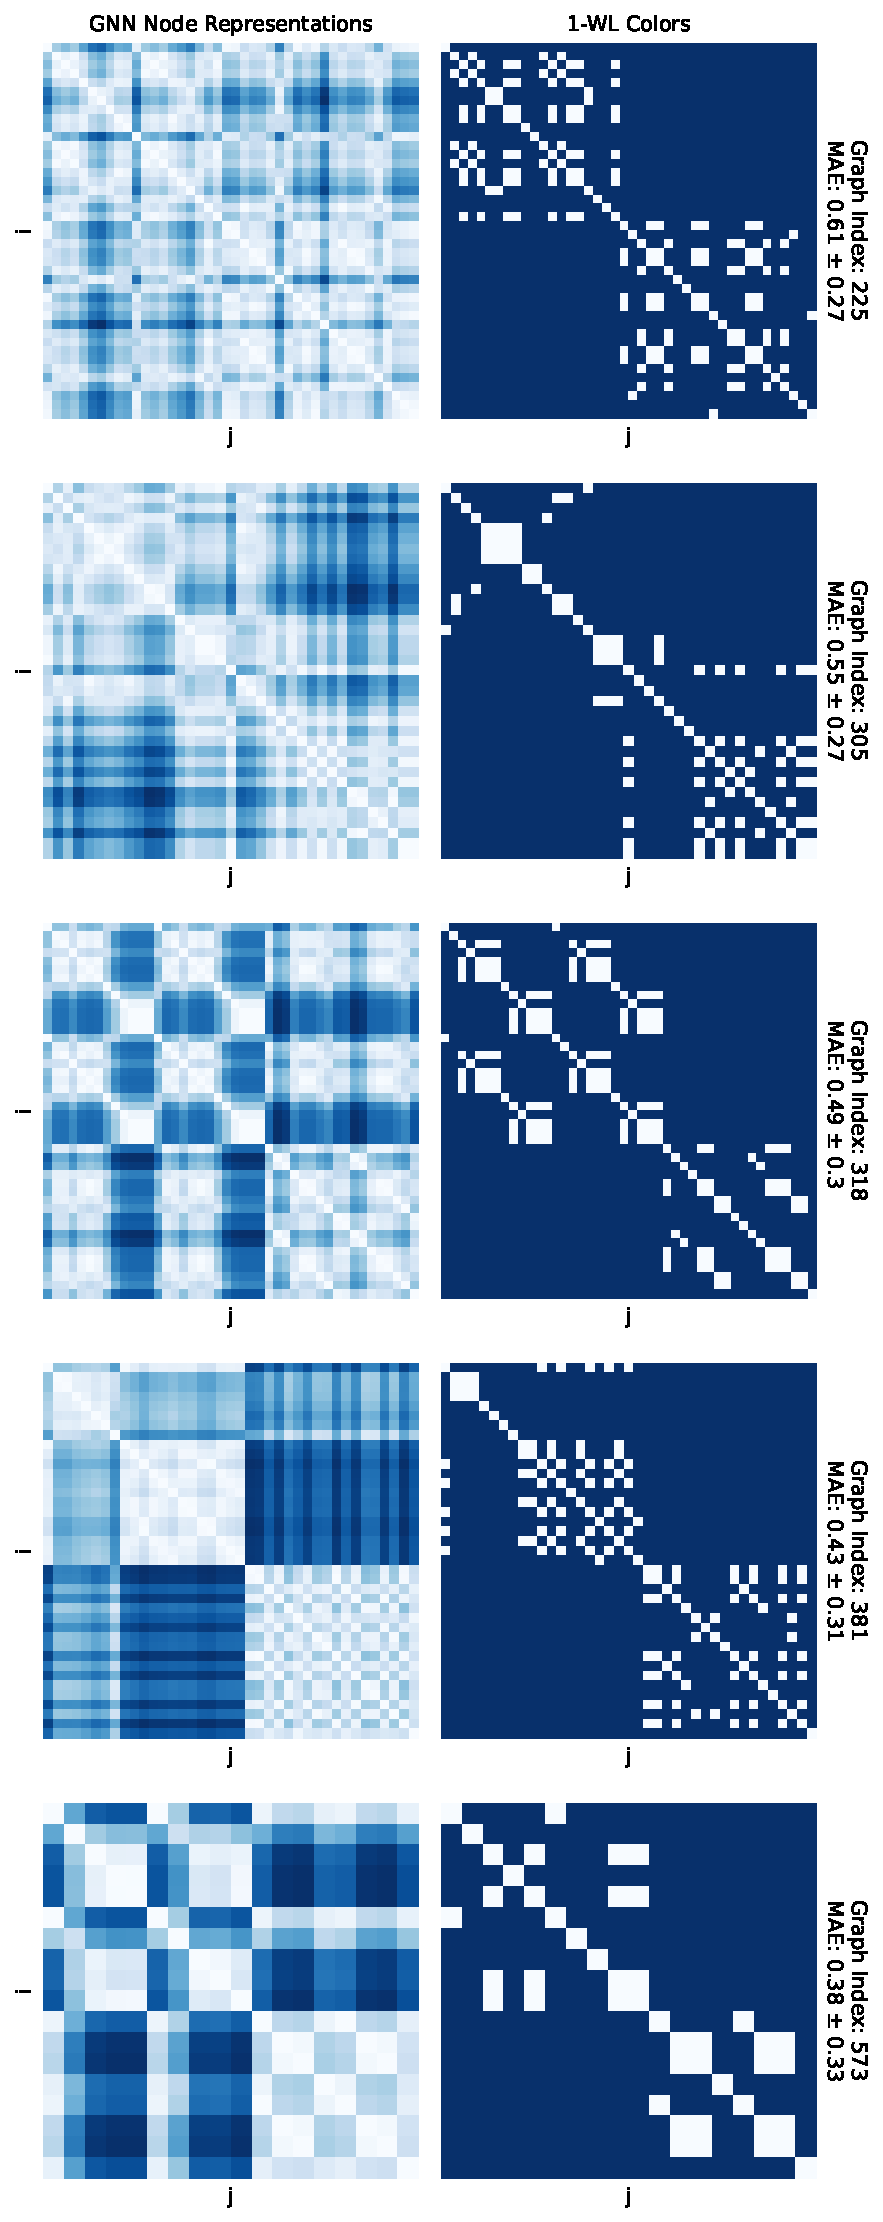
\includegraphics[width=\textwidth, left]{Figures/heatmaps_ENZYMES_0.pdf}
    \end{minipage}
    \hfill
    \begin{minipage}[b]{0.53007147296\textwidth}
        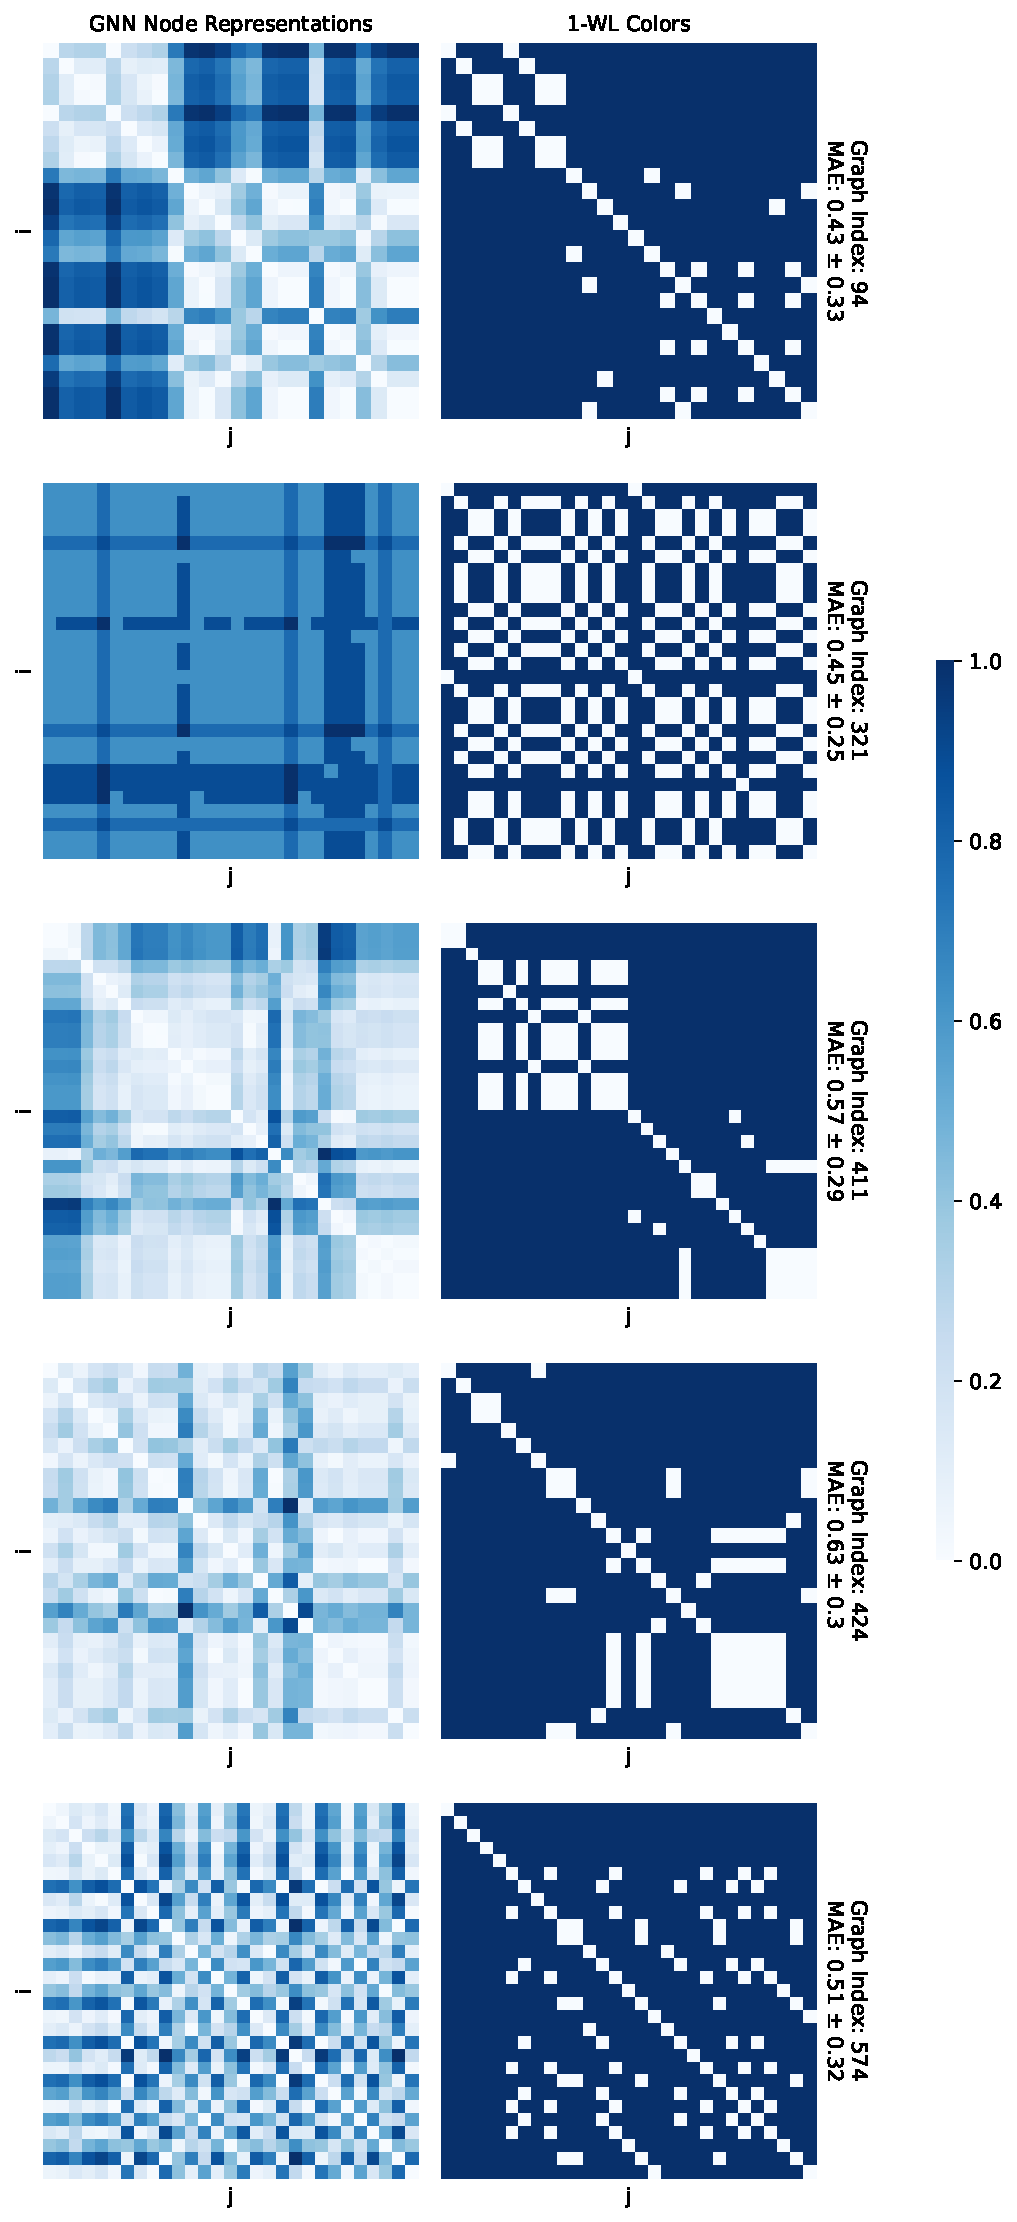
\includegraphics[width=\textwidth, right]{Figures/heatmaps_ENZYMES_1.pdf}
    \end{minipage}
    \hfill
    \caption{Visualizing the performance of the best performing GNN on the \textsc{Enzymes} dataset in approximating node colors computed by the 1-WL algorithm. The ten graphs shown are randomly sampled from the GNN's test set, and the 1-WL algorithm ran only for one iteration. The average error for the entire test set is $0.49 \pm 0.3$.}
\end{figure}

\begin{figure}[!ht]
    \centering
    \begin{minipage}[b]{0.45992852703\textwidth}
        \centering
        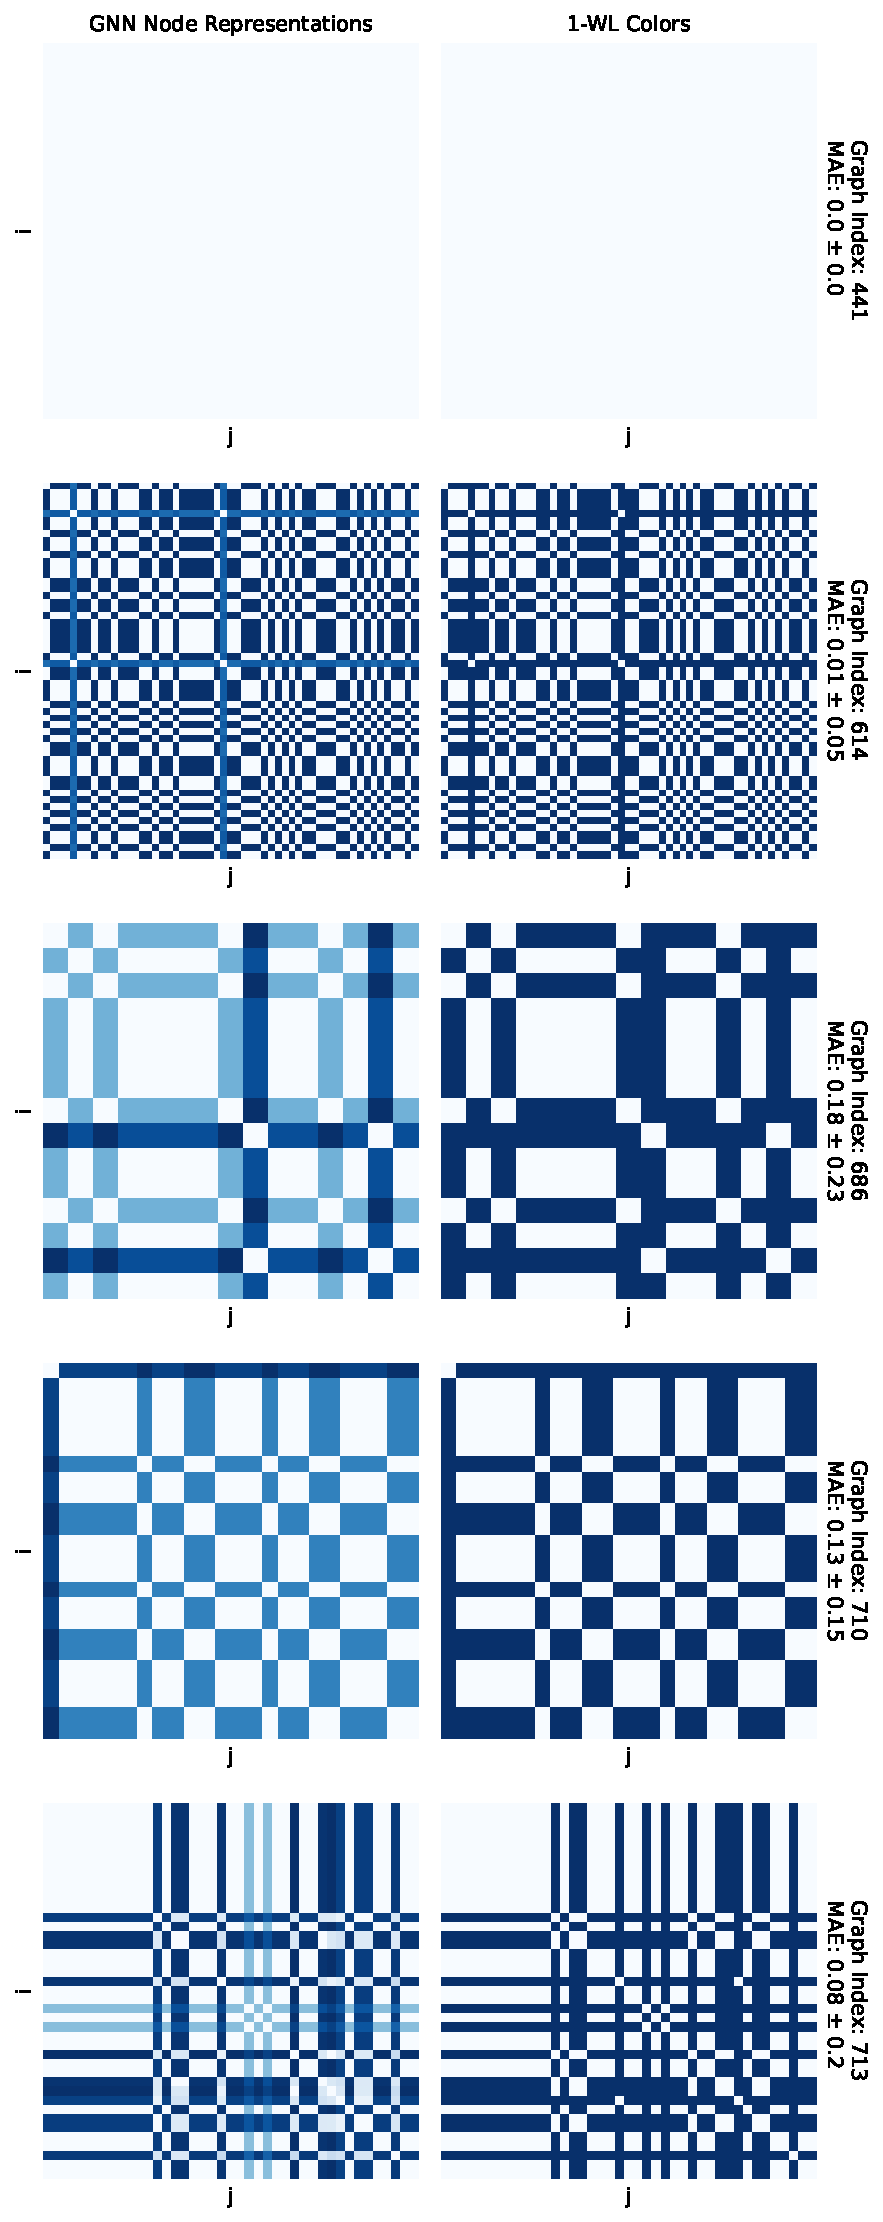
\includegraphics[width=\textwidth, left]{Figures/heatmaps_IMDB-BINARY_0.pdf}
    \end{minipage}
    \hfill
    \begin{minipage}[b]{0.53007147296\textwidth}
        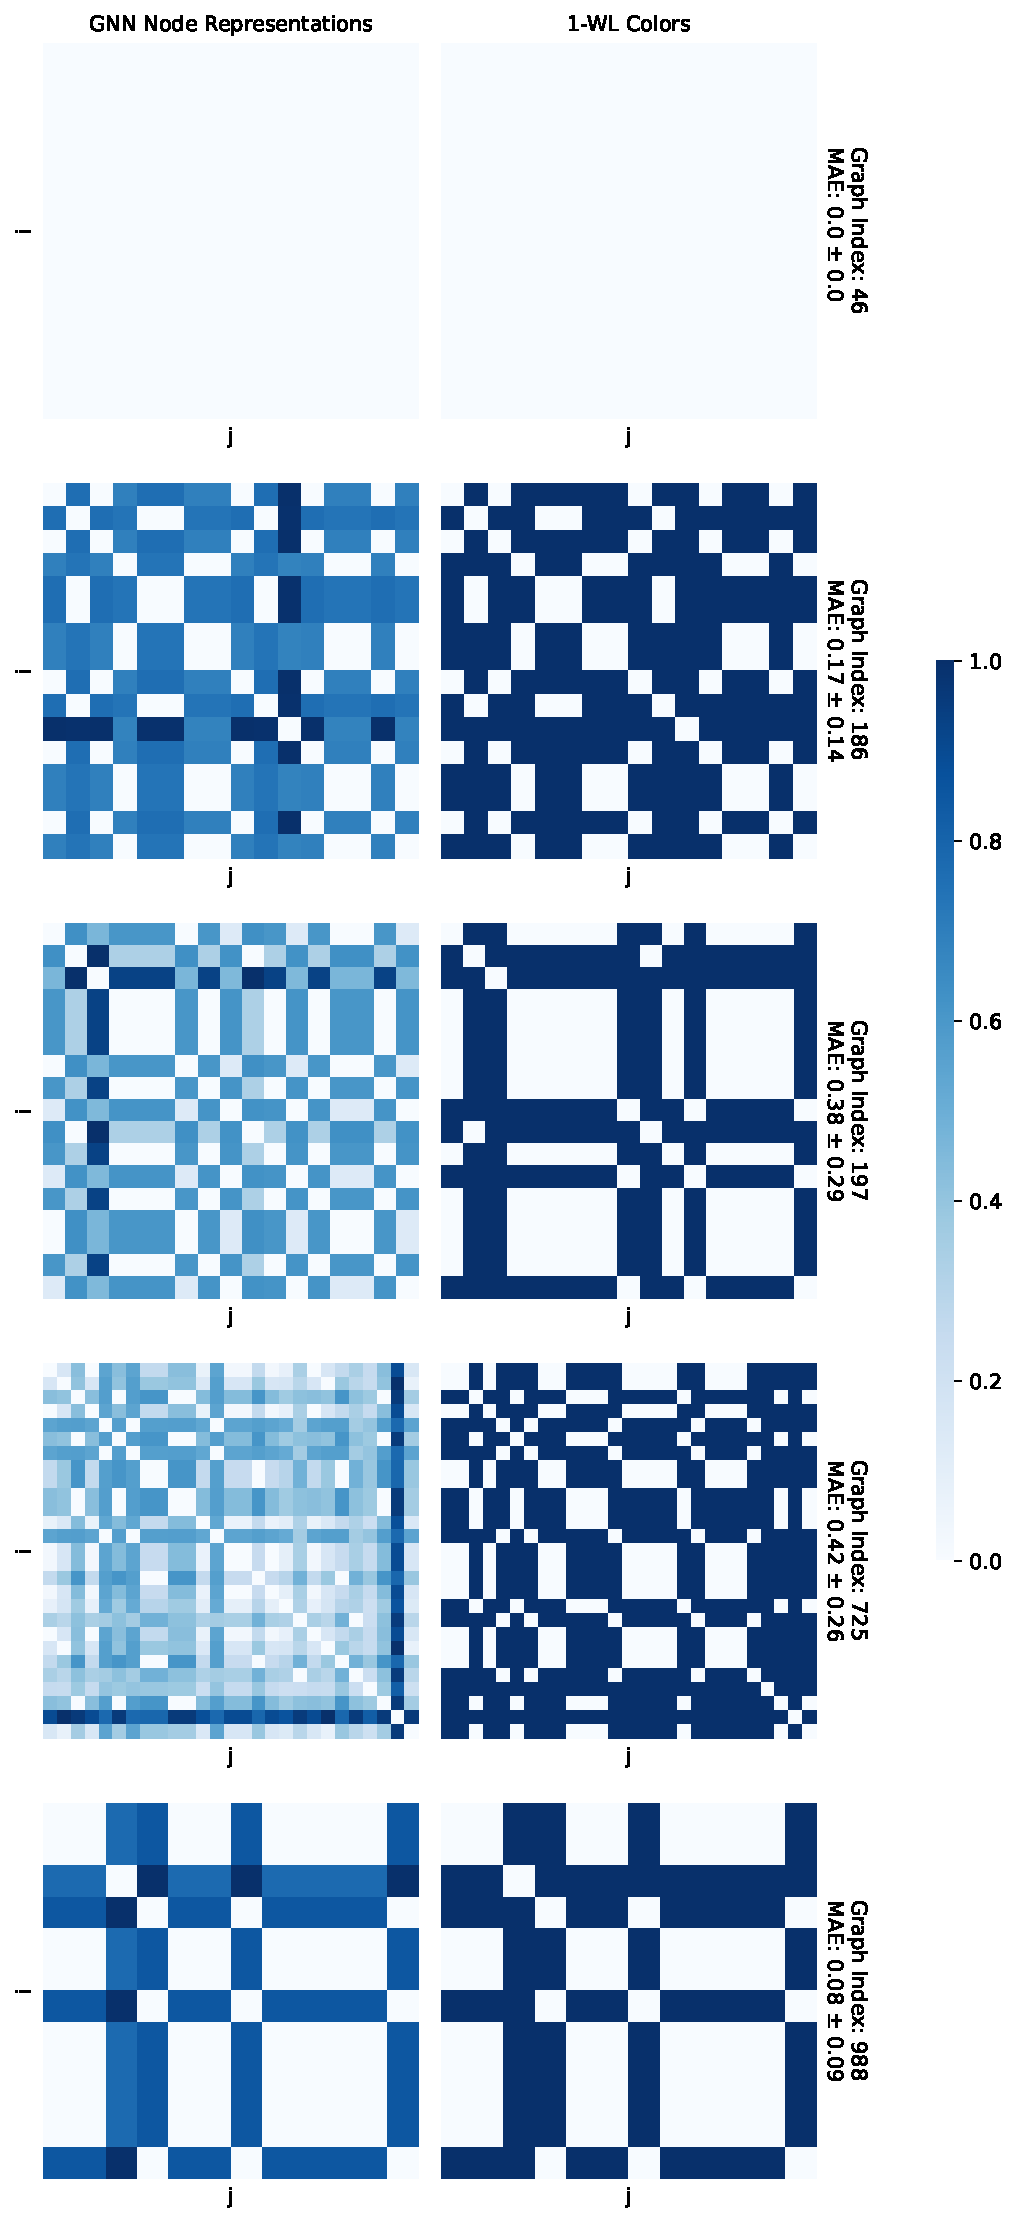
\includegraphics[width=\textwidth, right]{Figures/heatmaps_IMDB-BINARY_1.pdf}
    \end{minipage}
    \hfill
    \caption{Visualizing the performance of the best performing GNN on the \textsc{Imdb-Binary} dataset in approximating node colors computed by the 1-WL algorithm. The ten graphs shown are randomly sampled from the GNN's test set, and the 1-WL algorithm ran only for one iteration. The average error for the entire test set is $0.14 \pm 0.15$. \newline
    Note that \textsc{Imdb binary} does not contain any node features, so we artificially initialize each node feature with a one-hot encoding of its degree.}
\end{figure}

\begin{figure}[!ht]
    \centering
    \begin{subfigure}[b]{0.45992852703\textwidth}
        \centering
        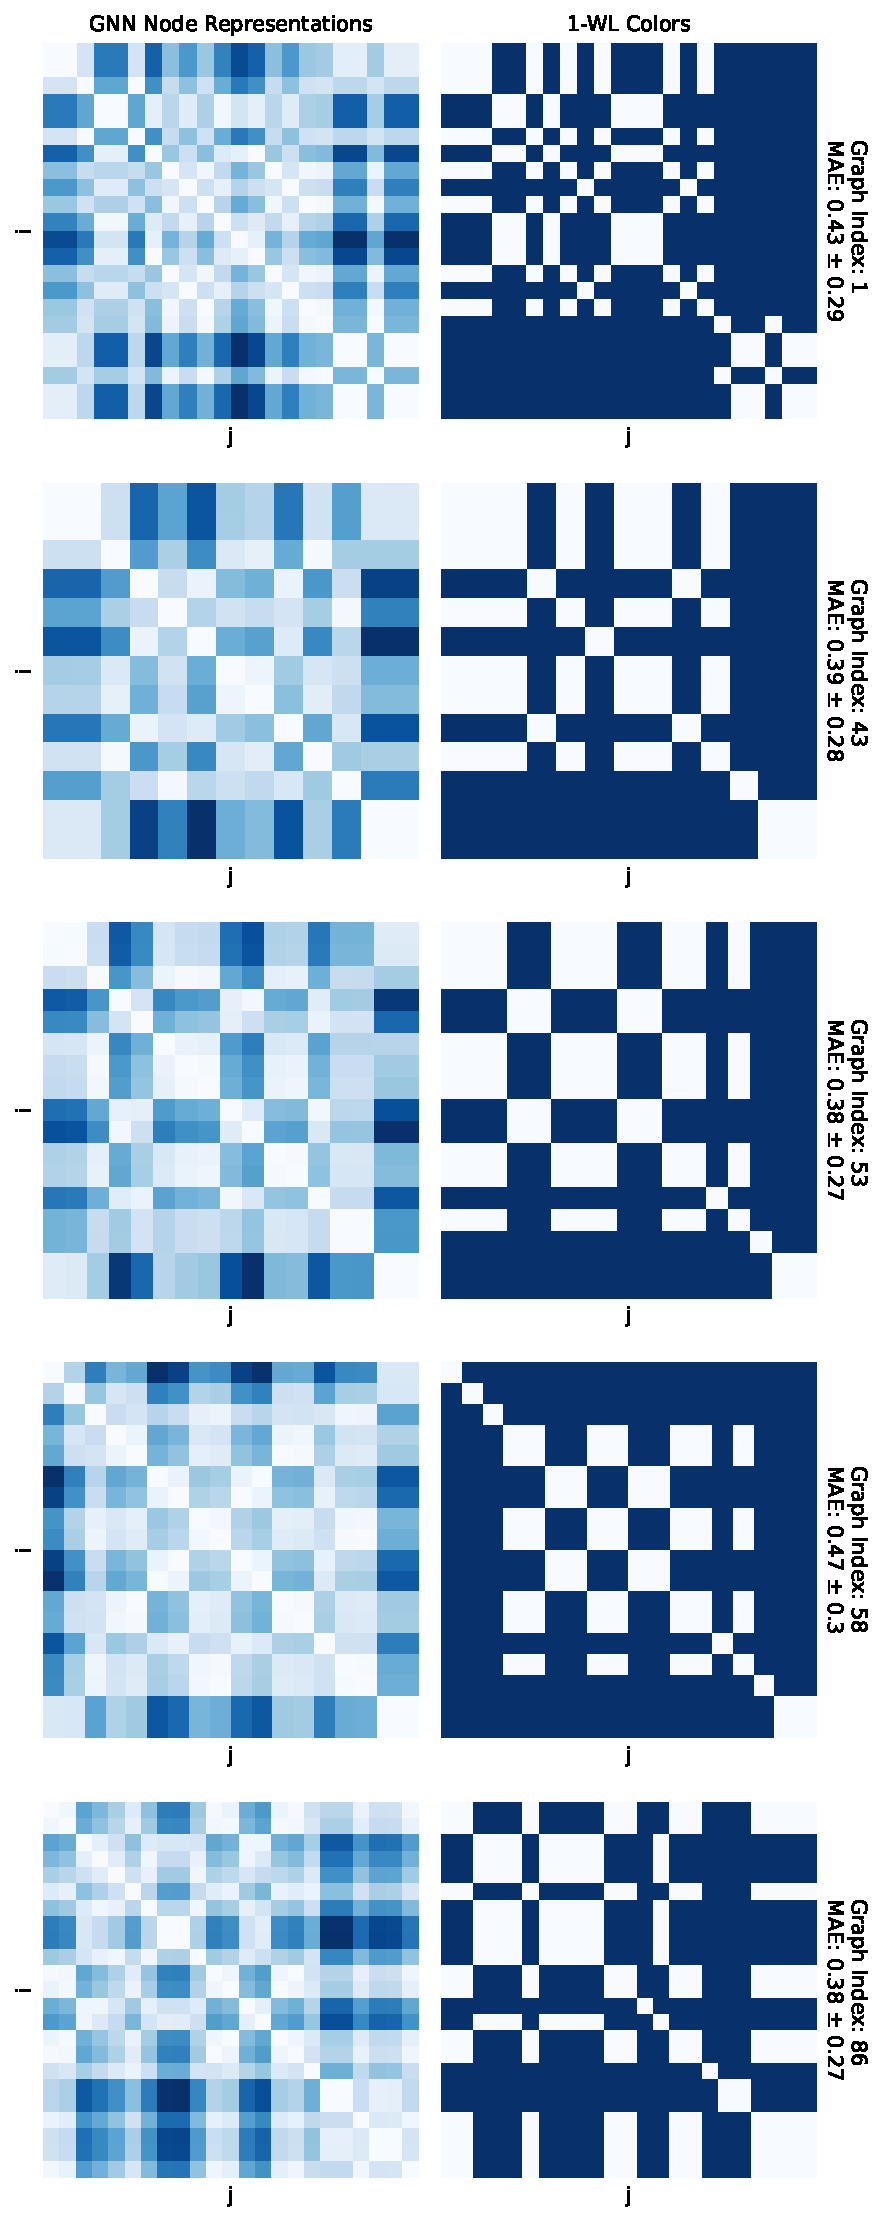
\includegraphics[width=\textwidth, left]{Figures/heatmaps_MUTAG_0.pdf}
    \end{subfigure}
    \hfill
    \begin{subfigure}[b]{0.53007147296\textwidth}
        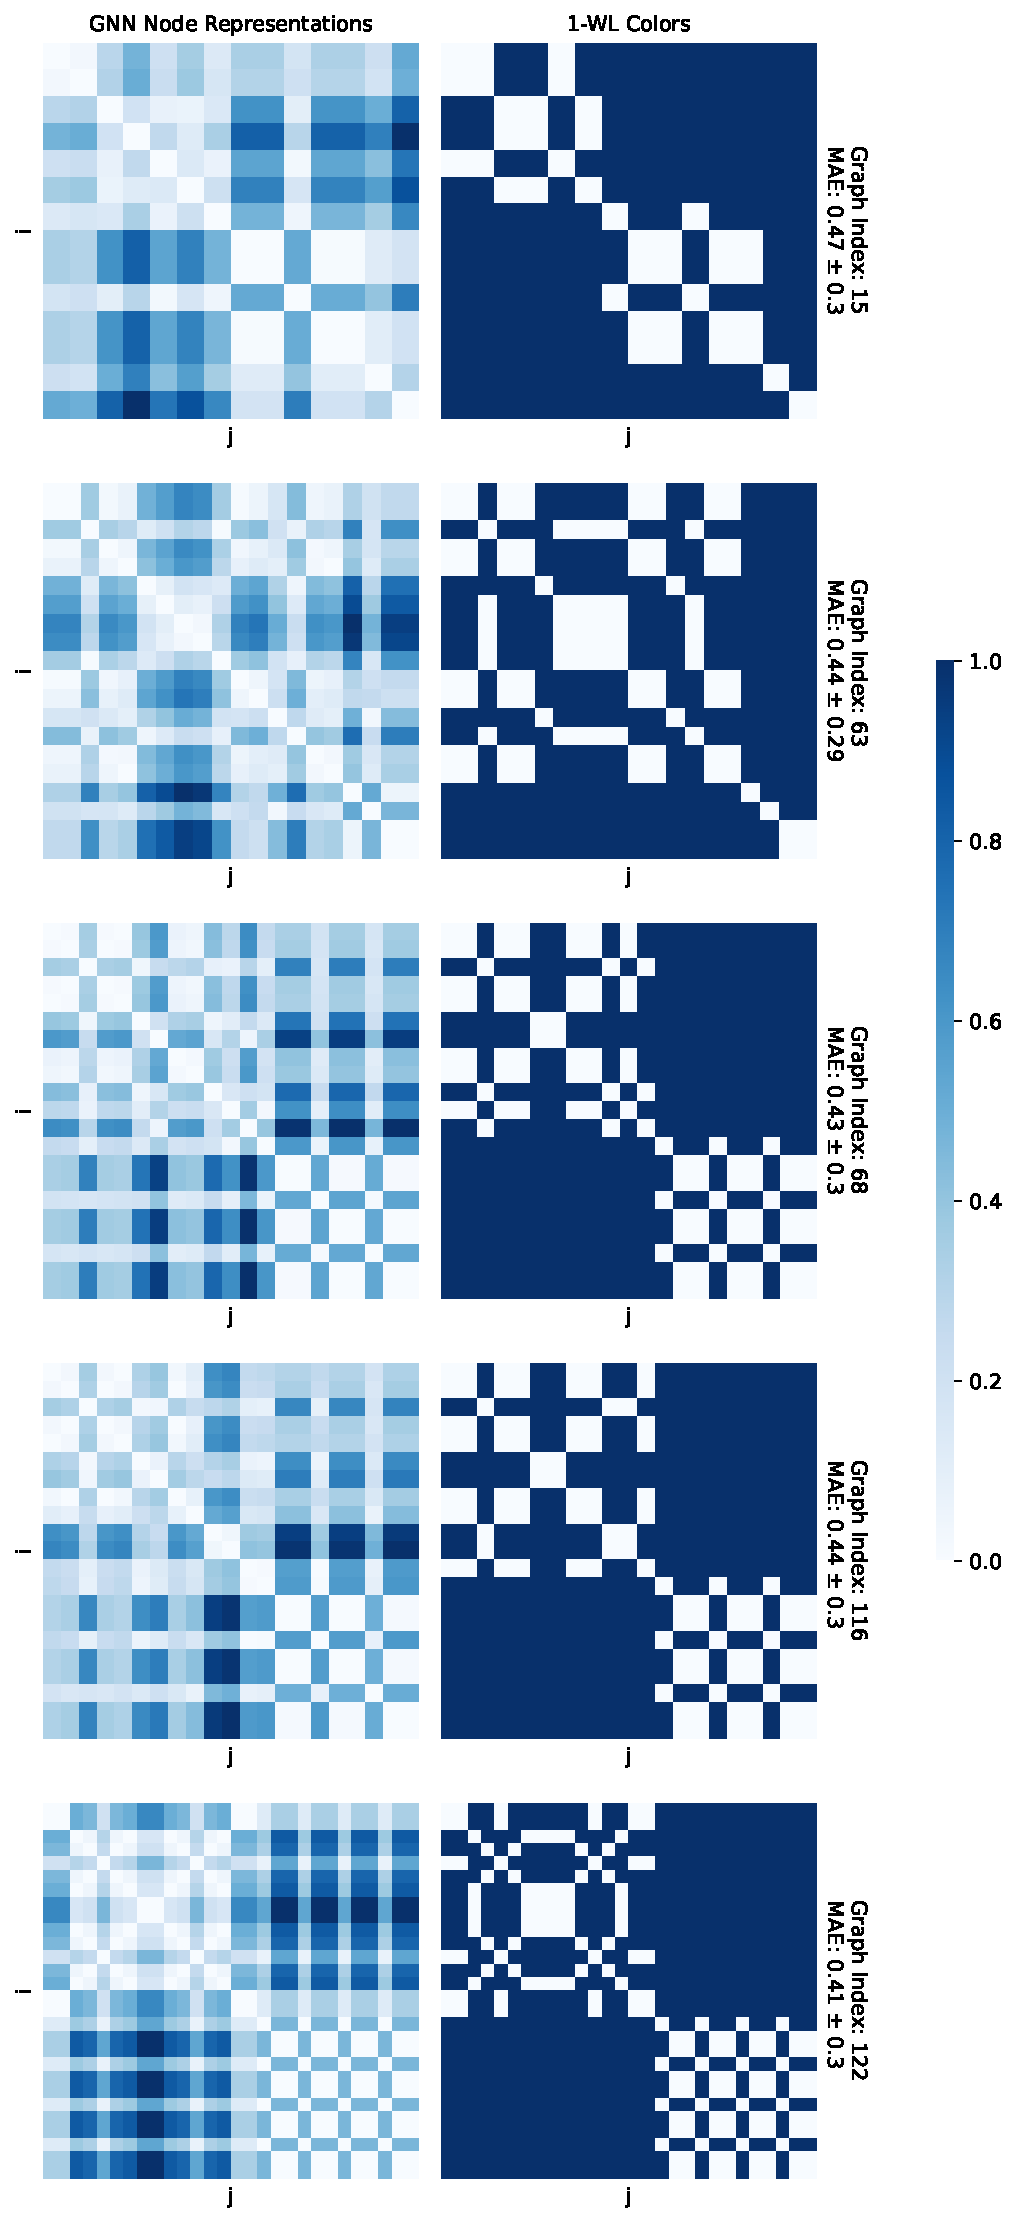
\includegraphics[width=\textwidth, right]{Figures/heatmaps_MUTAG_1.pdf}
    \end{subfigure}
    \hfill
    \caption{Visualizing the performance of the best performing GNN on the \textsc{Mutag} dataset in approximating node colors computed by the 1-WL algorithm. The ten graphs shown are randomly sampled from the GNN's test set, and the 1-WL algorithm ran only for three iteration. The average error for the entire test set is $0.42 \pm 0.29$.}
\end{figure}

\begin{figure}[!ht]
    \centering
    \begin{minipage}[b]{0.45992852703\textwidth}
        \centering
        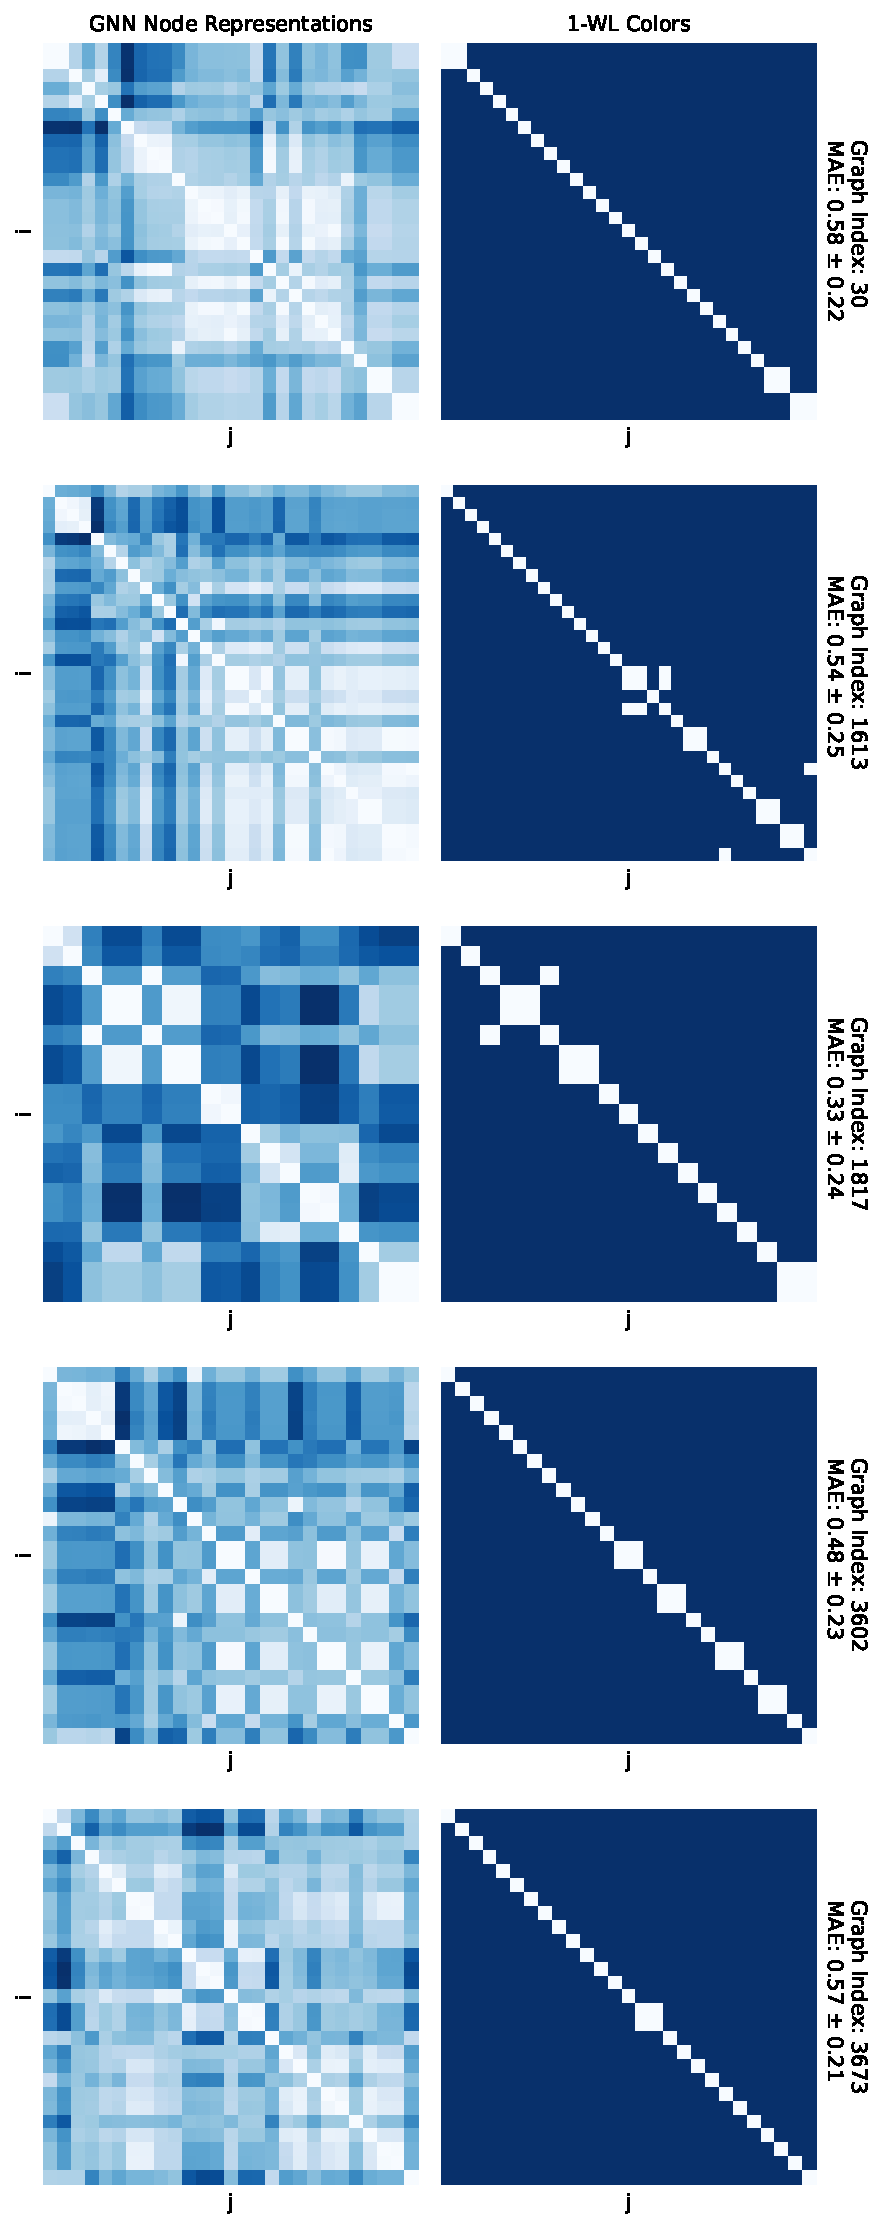
\includegraphics[width=\textwidth, left]{Figures/heatmaps_NCI1_0.pdf}
    \end{minipage}
    \hfill
    \begin{minipage}[b]{0.53007147296\textwidth}
        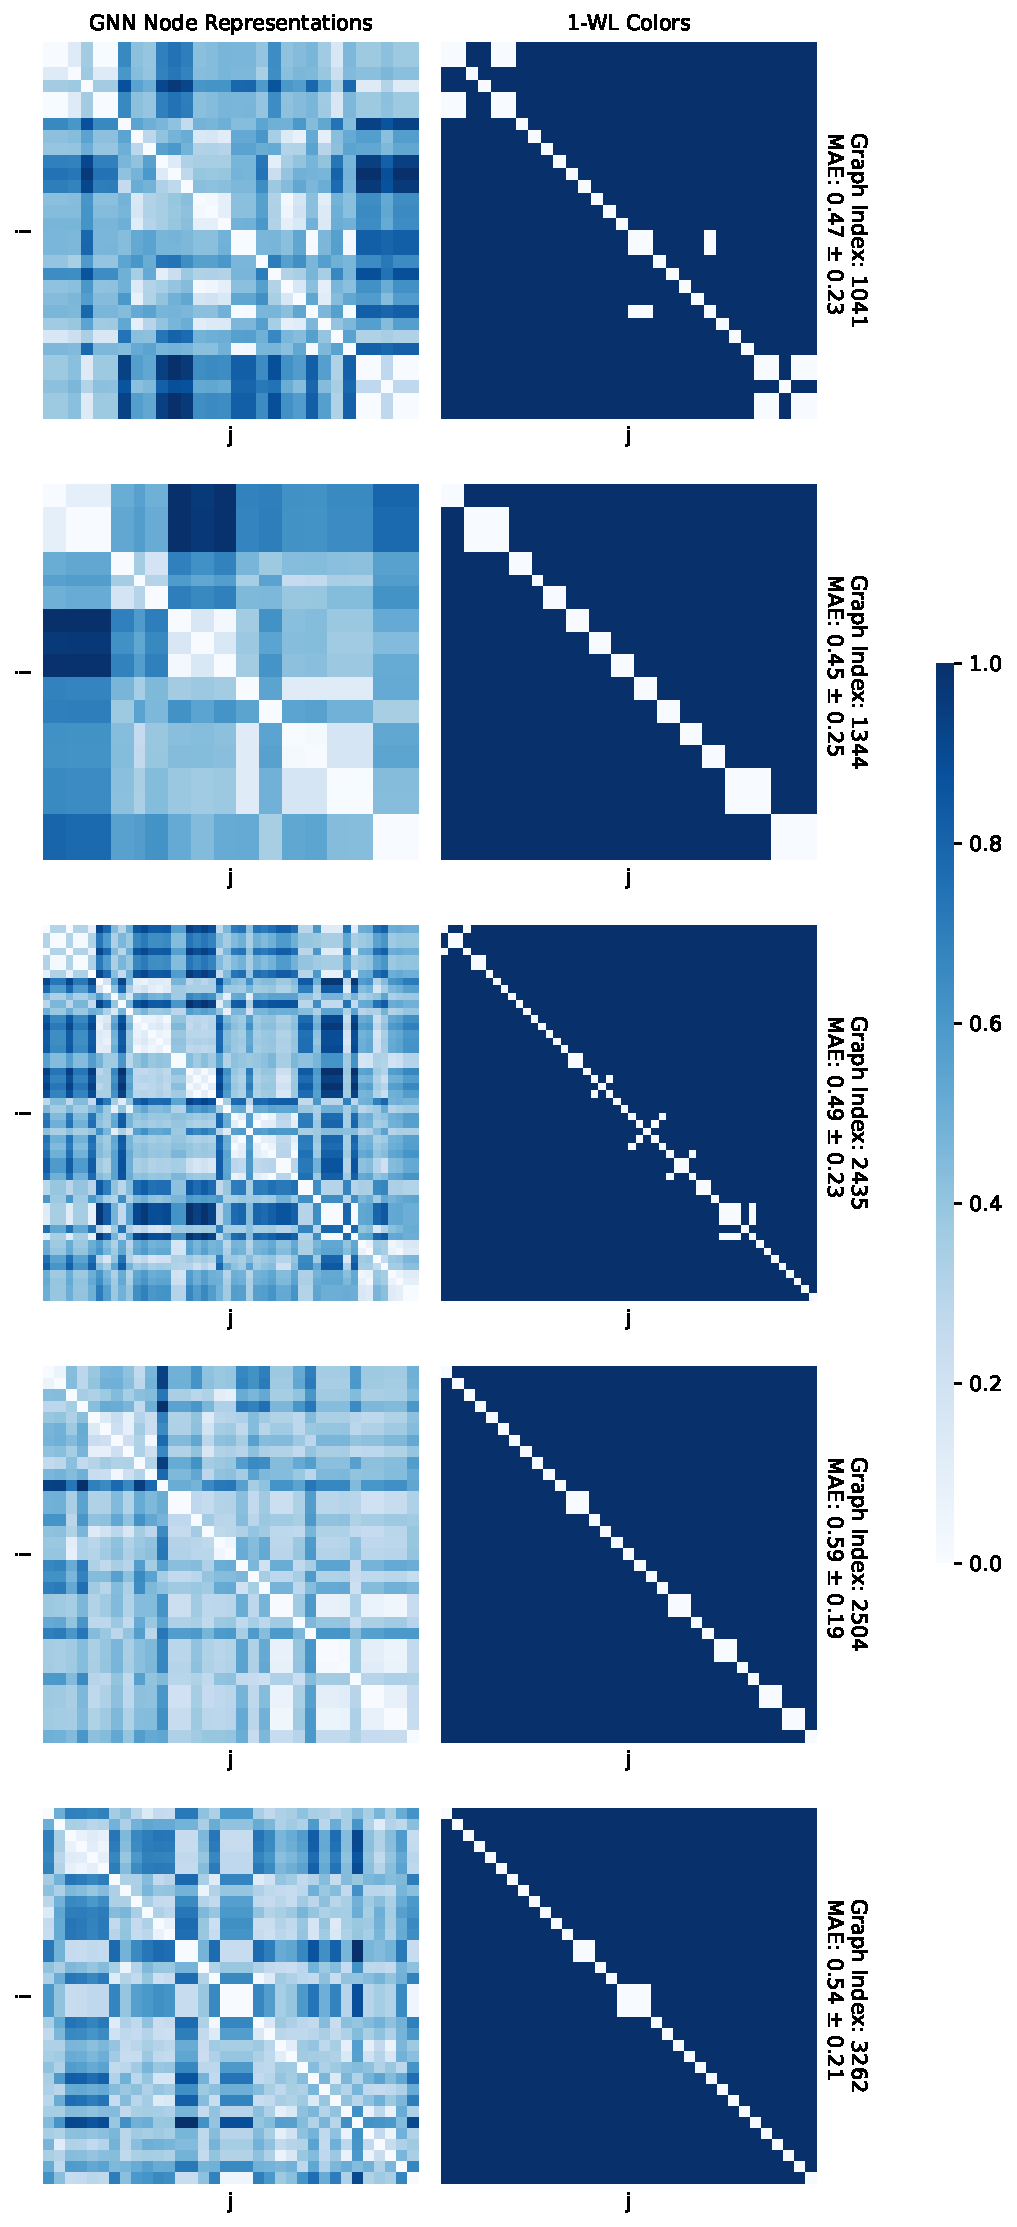
\includegraphics[width=\textwidth, right]{Figures/heatmaps_NCI1_1.pdf}
    \end{minipage}
    \hfill
    \caption{Visualizing the performance of the best performing GNN on the \textsc{Nci1} dataset in approximating node colors computed by the 1-WL algorithm. The ten graphs shown are randomly sampled from the GNN's test set, and the 1-WL algorithm ran only for three iteration. The average error for the entire test set is $0.50 \pm 0.24$.}
\end{figure}

\begin{figure}[!ht]
    \centering
    \begin{minipage}[b]{0.45992852703\textwidth}
        \centering
        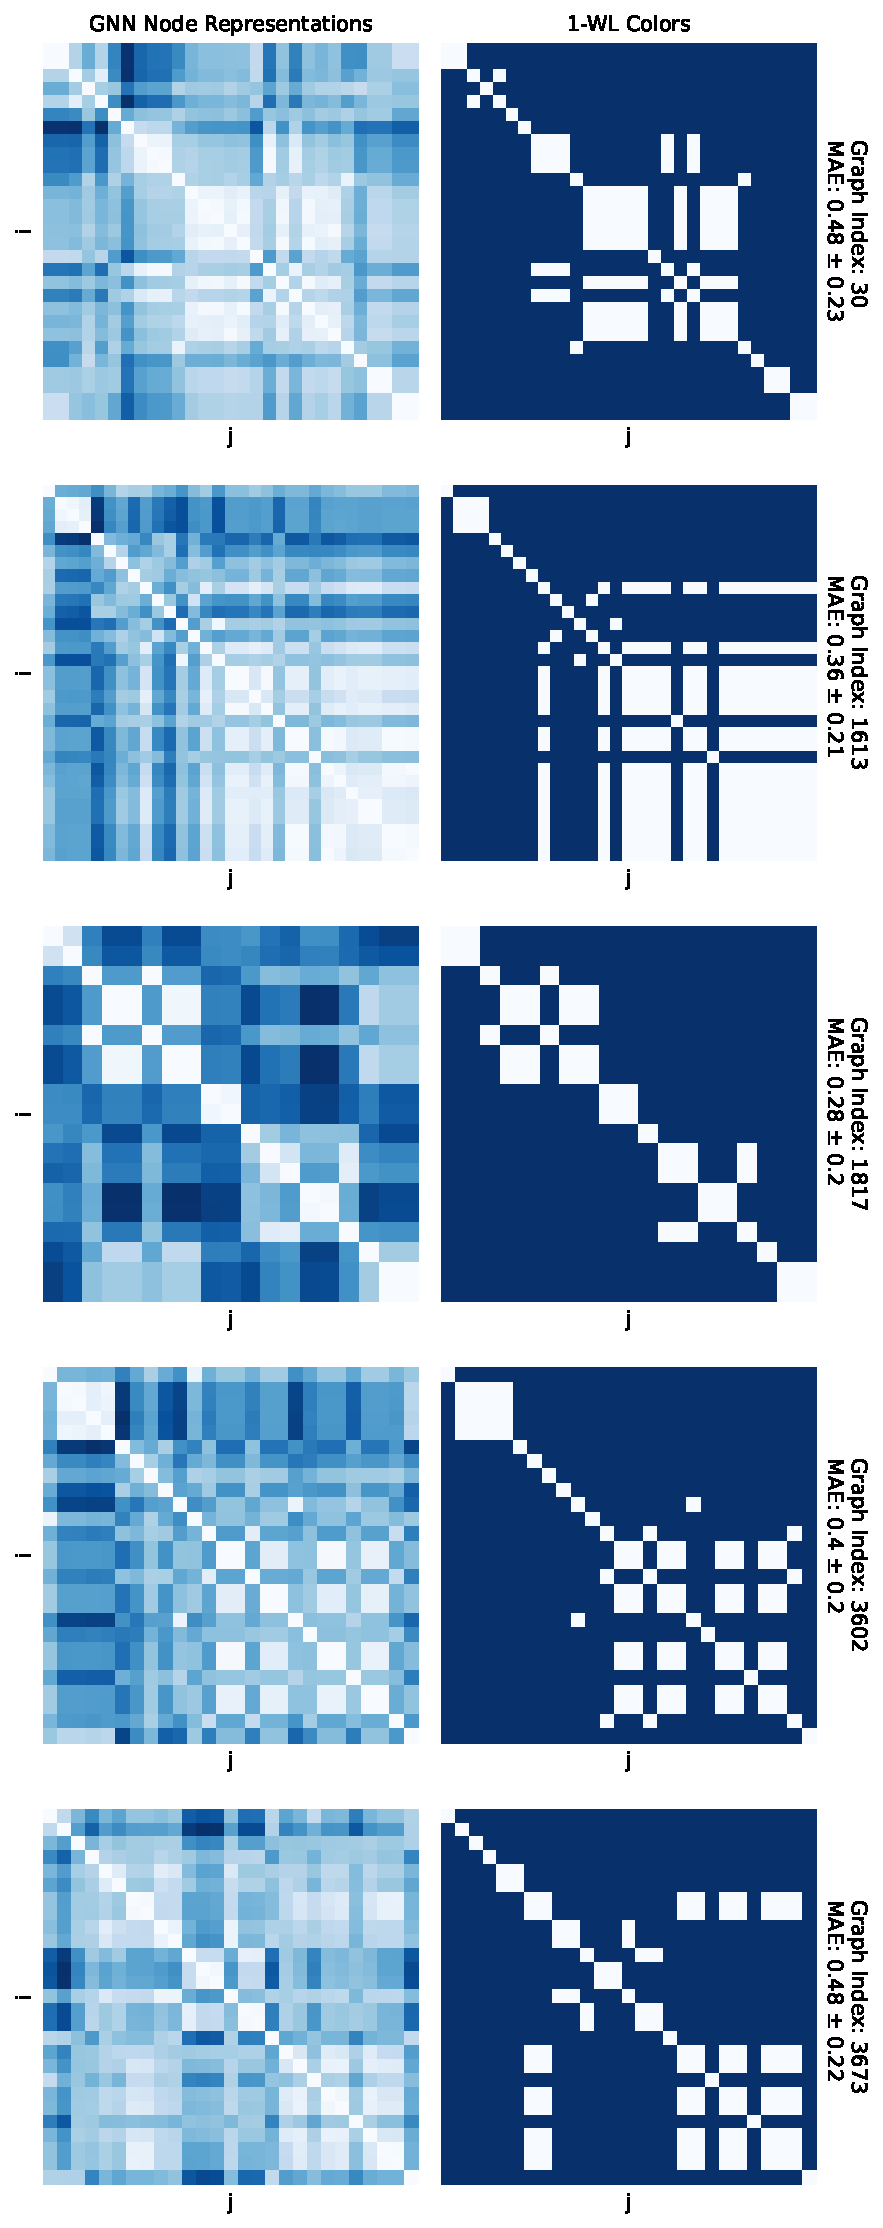
\includegraphics[width=\textwidth, left]{Figures/heatmaps_NCI1_0_k_wl_1.pdf}
    \end{minipage}
    \hfill
    \begin{minipage}[b]{0.53007147296\textwidth}
        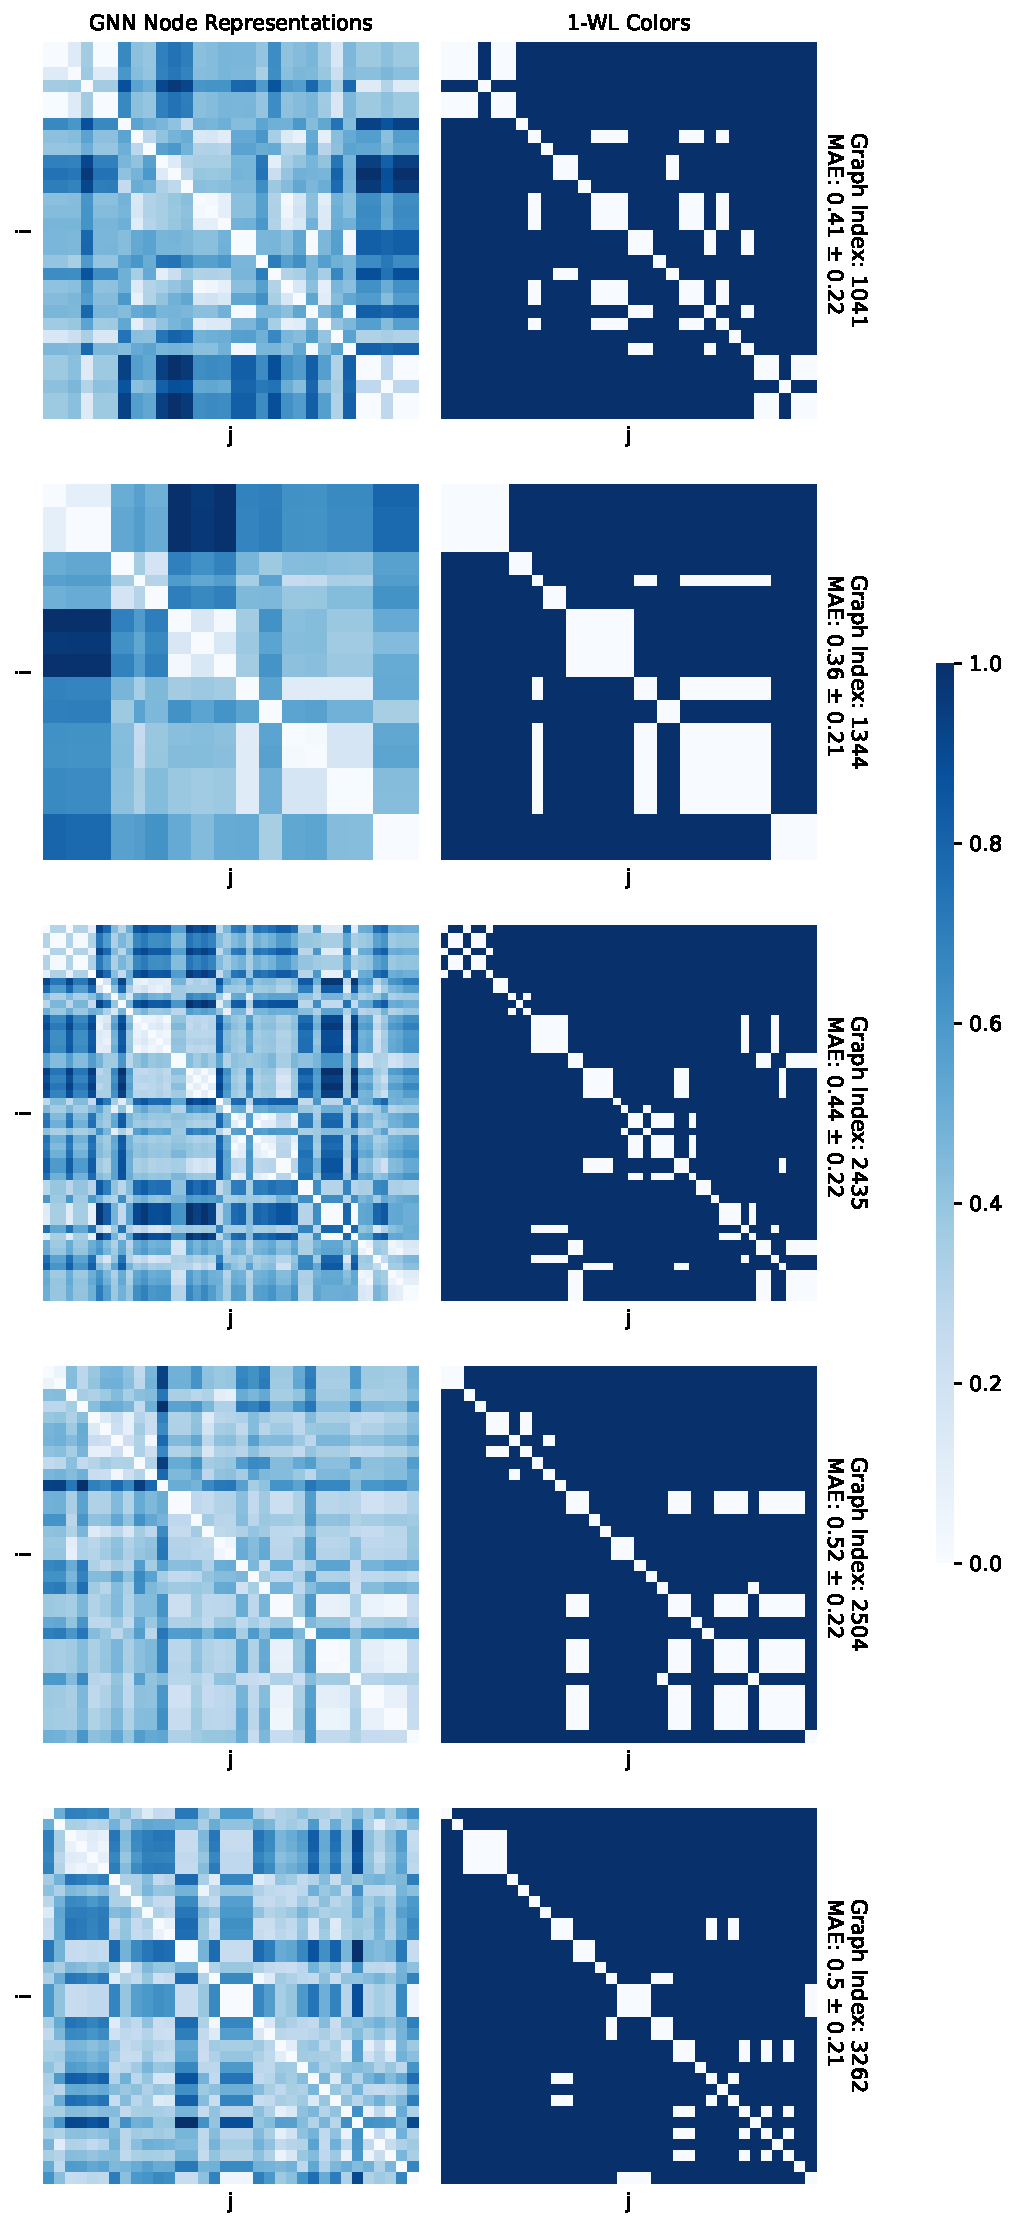
\includegraphics[width=\textwidth, right]{Figures/heatmaps_NCI1_1_k_wl_1.pdf}
    \end{minipage}
    \hfill
    \caption{Visualizing the performance of the best performing GNN on the \textsc{Nci1} dataset in approximating node colors computed by the 1-WL algorithm. The ten graphs shown are randomly sampled from the GNN's test set, and the 1-WL algorithm ran only for one iteration. The average error for the entire test set is $0.42 \pm 0.22$.}
\end{figure}

\begin{figure}[!ht]
    \centering
    \begin{minipage}[b]{0.45992852703\textwidth}
        \centering
        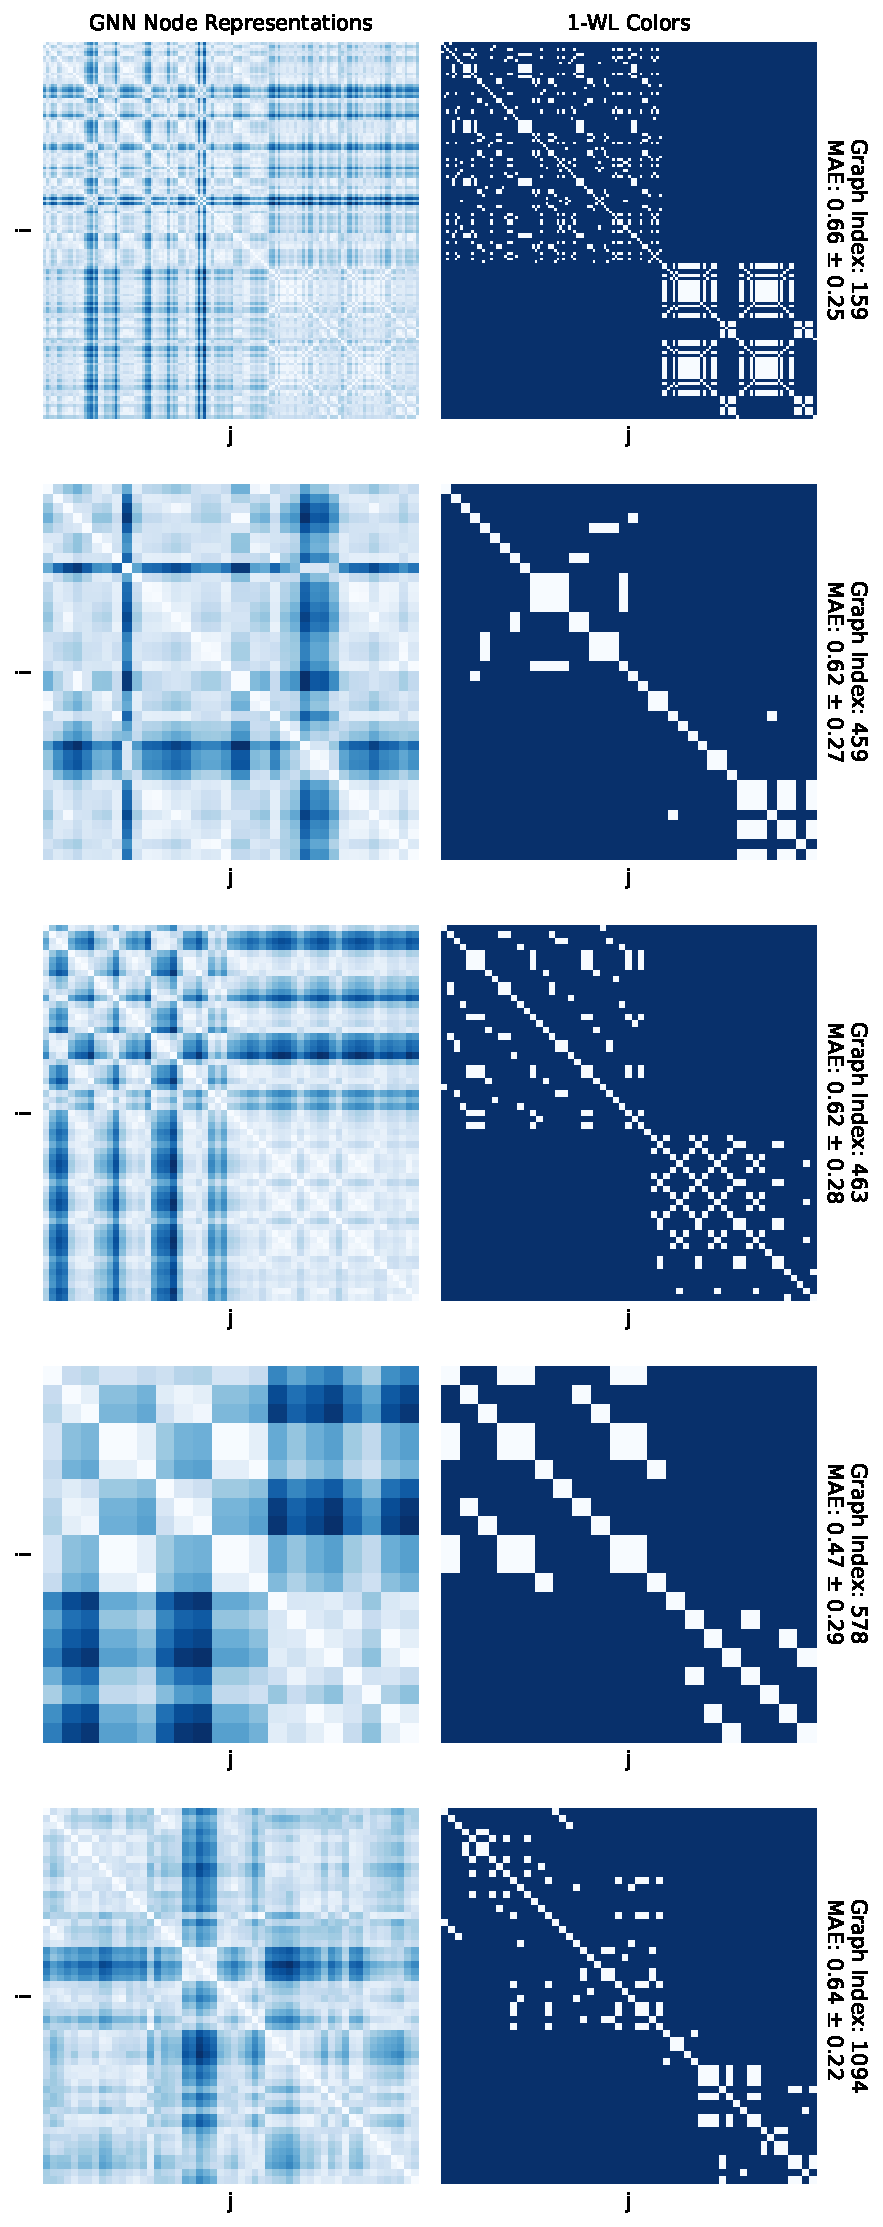
\includegraphics[width=\textwidth, left]{Figures/heatmaps_PROTEINS_0.pdf}
    \end{minipage}
    \hfill
    \begin{minipage}[b]{0.53007147296\textwidth}
        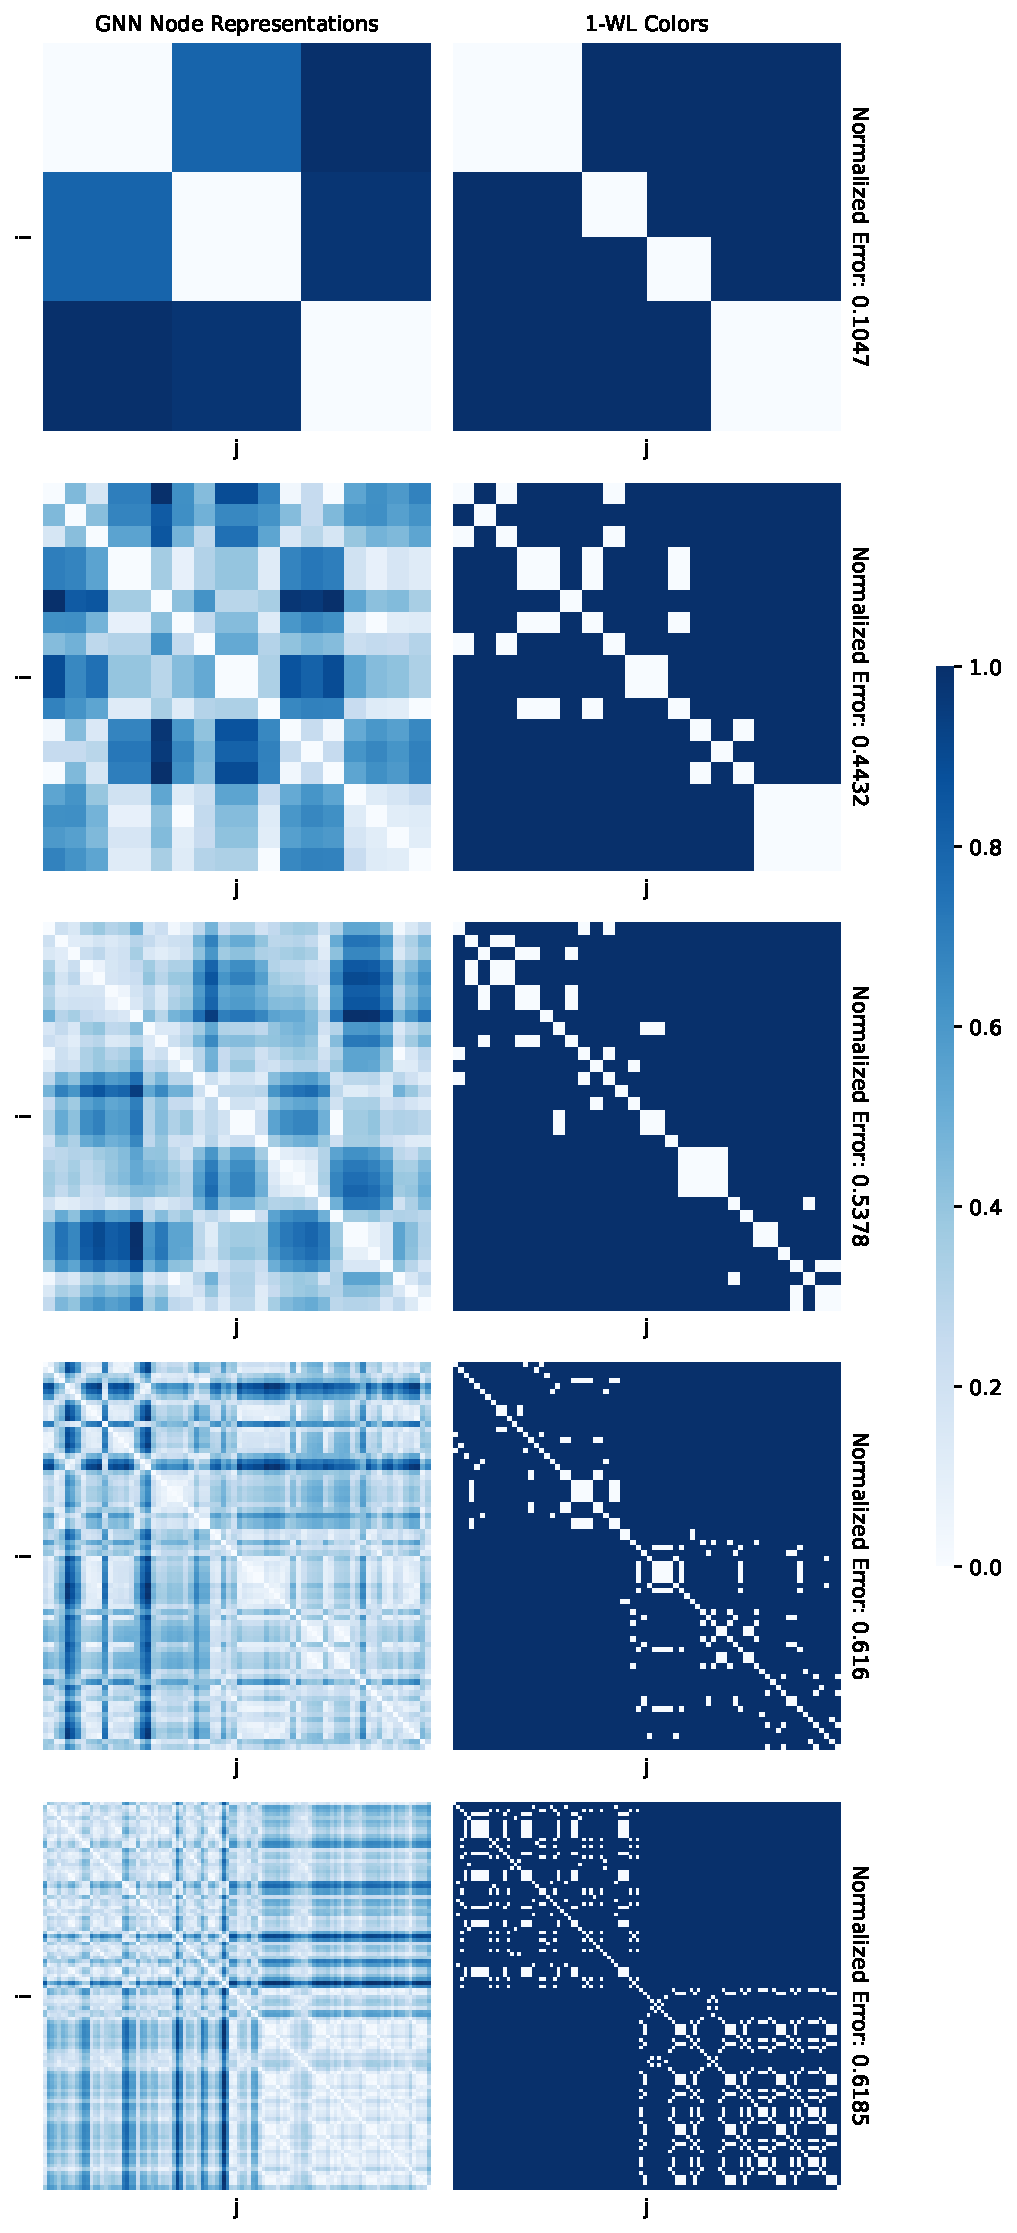
\includegraphics[width=\textwidth, right]{Figures/heatmaps_PROTEINS_1.pdf}
    \end{minipage}
    \hfill
    \caption{Visualizing the performance of the best performing GNN on the \textsc{Proteins} dataset in approximating node colors computed by the 1-WL algorithm. The ten graphs shown are randomly sampled from the GNN's test set, and the 1-WL algorithm ran only for one iteration. The average error for the entire test set is $0.49 \pm 0.26$.}
\end{figure}